\section{Problem 4: Design for Priority Model}
\subsection{Construction of Priority Model}
Generally speaking, the average income of long-distance taxis is higher than that of short-distance taxis. Therefore, the following priority schemes are formulated for short-distance taxis:

A short Lane will be added in the queuing area for taxis with short-distance passengers delivering last time. The other is the general queuing lane. The vehicles in the short Lane have priority to enter the loading area for reaching passengers, and the vehicles in the general lane can only enter the loading area for boarding passengers after all the vehicles in the short Lane have been arranged. Every time the taxi finishes loading passengers from the airport, there will be mileage record. When the airport staff determines that the mileage record is a short distance, the taxi can enter the short distance lane for priority.

The following analysis shows the change of taxi revenue after the implementation of the plan:

Assume the short-distance taxis returns to the airport every time after delivering short-distance passengers. They start to line up at time $D$, board at time $E$, finish delivering at time $F$, return to the airport at time $G$. The short-distance taxis continuously delivering the short-distance passengers $i$ times in a cycle until get and deliver long-distance passenger, then the total revenue of the short-distance taxis is:
\begin{equation}
	W_{st} = I_{s} \cdot i + I_{l}, i = 1,2,3,..,N_{c}
\label{W_st}
\end{equation}
where $I_{s}$ and $I_{l}$ are the short-distance and long-distance taxi fares respectively, which are determined by the taxi charging standard and the mileage $L_{s}$ and $L_{l}$, and the net income is:
\begin{equation}
	W_{s} = W_{st} - 2 \cdot o \cdot i + O_{l}
\label{W_s}
\end{equation}
$O_{s}$ and $O_{l}$ are respectively the fuel charge for short-distance and long-distance mileage:
\begin{equation}
	O_{s} = o \cdot k + L_{s}
\label{O_s}
\end{equation}
\begin{equation}
	O_{l} = o \cdot k + L_{l}
\label{O_l}
\end{equation}
The probability that the taxi will carry the short distance passengers for $i-1$ times after the first time is:
\begin{equation}
	P(x = i)=(1-P_{l})^{i-1}\cdot P_{l}
\label{P_i}
\end{equation}
Obviously, the random variable $i$ obeys the geometric distribution. Its expectation is:
\begin{equation}
	E(X)=\frac{1}{P_{l}}
\label{E_X}
\end{equation}
The total cycle time is the time of $i$ times queues, plus the time of $i$ round trips, plus the time of the last long-distance delivery:
\begin{equation}
	t_{s2} = t_{DE} \cdot i + 2 \cdot i \cdot t_{EF} + t_{l}
\label{t_s2}
\end{equation}
$t_{EF}$ and $t_{L}$ are also related to mileage $L_{s}$ and $L_{L}$, respectively:
\begin{equation}
	t_{EF} = \frac{L_{s}}{\alpha \cdot \beta \cdot V_{1}}
\label{t_EF}
\end{equation}
\begin{equation}
	t_{l} = \frac{L_{l}}{\alpha \cdot \beta \cdot V_{1}}
\label{t_l}
\end{equation}
$t_{DE}$ is obtained by clustering analysis of flight density and taxi density in this time period. So the average hourly revenue of short distance vehicles in the cycle becomes:
\begin{equation}
	\bar{W_{s}} = \frac{I_{s}\cdot E(X)+I_{l}-2\cdot O_{s}\cdot E(X)-O_{l}}{t_{DE} \cdot E(X)+2 \cdot E(X)\cdot t_{EF}+t_{l}}
\label{W_s_bar}
\end{equation}
It is set that the long-distance taxis will not return to the airport after delivering passengers. For the long-distance bus, one cycle is queuing, carrying and finishing delivering. Assume the long-distance taxis start to queue at time $D$, carry passengers at time $E$ (the average queuing time of all the taxis is the same), and carry passengers at time $H$, then the average hourly income $\bar{W_{l}}$ of the long-distance taxi meets the requirements:
\begin{equation}
	\bar{W_{l}} = \frac{I_{l}-O_{l}}{t_{DE} +t_{EH}}
\label{W_l_bar}
\end{equation}
where
\begin{equation}
	O_{l} = o \cdot k + L_{l}
\label{O_l}
\end{equation}
\begin{equation}
	t_{EH} = t_{l}
\label{t_EH}
\end{equation}
Set the total number of taxis is $N_{C}$, and the proportion of long-distance vehicles is $P_{l}$. then, the average hourly income $W_{b}$ for every taxi  before the implementation of the plan is:
\begin{equation}
	W_{b} = \bar{W_{l}}\cdot P_{l} + \bar{W_{s}} \cdot (1 - P_{l})
\label{W_b}
\end{equation}
The variance of the average revenue is:
\begin{equation}
	S_{b} = N_{c}\cdot P_{l}\cdot (\bar{W_{l}} - W_{b})^{2} + N_{c}\cdot(1- P_{l}) \cdot (\bar{W_{s}} - W_{b})^{2}
\label{S_b}
\end{equation}
After the implementation of the plan, the cycle of the short distance vehicle is still $i$ consecutive short distance cycle plus the last long distance cycle, and its net income is the same as before the implementation of the plan:
\begin{equation}
	W_{s2} = W_{s}
\label{W_s2}
\end{equation}
After the first queue, the time of each queue is decreased, changes to:
\begin{equation}
	t_{DE2} = (1-P_{l})\cdot t_{DE}
\label{t_DE2}
\end{equation}
The total cycle time is the time of the first queue plus the time of the next $i-1$ queues plus the time of $i$ round trips plus the time of the last long-distance delivery:
\begin{equation}
	t_{s2} = t_{DE}+t_{DE2}\cdot (i-1) + 2 \cdot i \cdot t_{EF} + t_{EH}
\label{t_s2}
\end{equation}
So the average hourly revenue of short distance vehicles in the cycle becomes:
\begin{equation}
	\bar{W_{s2}} = \frac{I_{s}\cdot E(X)+I_{l}-2\cdot O_{s}\cdot E(X)-O_{l}}{t_{DE} +t_{DE2}\cdot (E(X)-1)+2 \cdot E(X)\cdot t_{EF}+t_{EH}}
\label{W_s_2}
\end{equation}
For a long-distance taxi, still assume the long-distance taxi does not turn back to the airport, the average revenue of one cycle of the long-distance taxi is:
\begin{equation}
	\bar{W_{l2}} = \bar{W_{l}}
\label{W_l2_bar}
\end{equation}
The average hourly revenue per taxi becomes:
\begin{equation}
	W_{a} = \bar{W_{l2}}\cdot P_{l} + \bar{W_{s2}} \cdot (1 - P_{l})
\label{W_a}
\end{equation}
The variance of revenue becomes:
\begin{equation}
	S_{a} = N_{c}\cdot P_{l}\cdot (\bar{W_{l2}} - W_{a})^{2} + N_{c}\cdot(1- P_{l}) \cdot (\bar{W_{s2}} - W_{a})^{2}
\label{S_b}
\end{equation}
If $S_{b}$ > $S_{a}$, it shows that our priority scheme does make the revenue of all taxis in this time period more balanced.
\subsection{Verification of Priority Model}
Similarly, Pudong Airport is selected as the actual example. The scenario is the same as the previous example with the same parameter setting of table\ref{parameter_setting}. 

For the time being, the value of $P_{l}$ cannot be obtained. Therefore, we have set multiple candidate values for $P_{l}: 0.6, 0.7, 0.8$, (set $P_{l} > 0.5$, because most airport passengers are long-distance passengers) and we observed multiple experimental results. And from these results, we can draw some conclusions:
\begin{figure}[h]
\centering
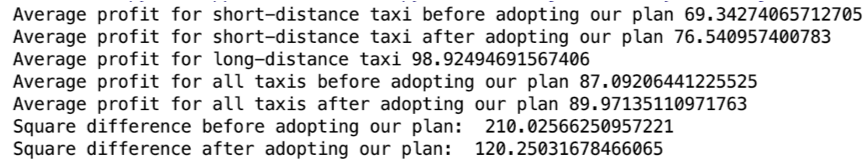
\includegraphics[width = 1.0\textwidth]{P_l6.png}
\caption{Results when $P_{l} = 0.6$}
\label{P_l6}
\end{figure}

\begin{figure}[h]
\centering
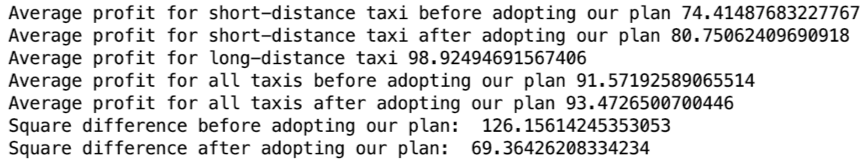
\includegraphics[width = 1.0\textwidth]{P_l7.png}
\caption{Results when $P_{l} = 0.7$}
\label{P_l7}
\end{figure}

\begin{figure}[h]
\centering
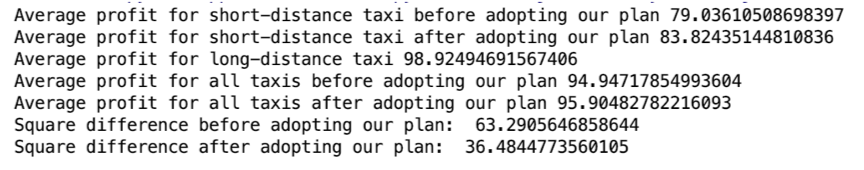
\includegraphics[width = 1.0\textwidth]{P_l8.png}
\caption{Results when $P_{l} = 0.8$}
\label{P_l8}
\end{figure}

\begin{enumerate}

\item 
This scheme can significantly reduce the variance of average revenue and make the revenue of all taxis as balanced as possible.
\item 
It is true that airport long-distance passenger transport is more profitable than short-distance passenger transport, so it is a scientific and reasonable measure to set up a priority scheme for short-distance vehicles.
\item
This scheme improves the average revenue of short distance vehicles and all taxis to a certain extent.
\item
With the increase of $P_{l}$, almost all taxis take long-distance passengers, so the variance of the overall income decreases.
\end{enumerate}
%
%
%
%\subsection{Weaknesses}
%\begin{enumerate}
%\item \textbf{Our model is just a rough model} \\
%For simplicity, we have neglected many potential parameters, variables or processes, and have made numerous assumptions. Eg. we did not consider the relationship between separate individuals and we did not dig deeper into the properties of social network which is a quite essential part determining the spread of disease. Some important general or specific factors are also neglected by us, a interesting example of which is a folk custom prevalent in the studied region that relatives kiss the death, which plays a significant role in the spread of disease and is categorized into \emph{Super Spread Event}(SSE) academically. 
%
%\item \textbf{Our model is only a continuous model} \\
%Numbers of people, number of shares of drug/vaccine, etc. are important quantities in all the process of modeling and computation. For simplicity, we regard the numbers as directly real numbers instead of integers. It is justifiable when the numbers are large, since the decimal part of the number is negligible; when the system scales down, however, the statistics dose not work and the outcome deviates a lot from reality.
%\end{enumerate}